


\chapter{Van Allen Probe Observations}
  \label{ch_rbsp}

The results presented in \cref{ch_results} are interesting on their own, but
become particularly valuable when combined with observational data.
Unfortunately, only a small number of studies to date have explored how Pc4
observation rate is affected by the harmonic and polarization structure of
those waves. While Pc4 pulsations have previously been studied in terms of both
harmonic\cite{arthur_1981,cummings_1969,engebretson_1988,hughes_1978,
singer_1982,takahashi_1984} and 
polarization\cite{anderson_1990,dai_2015,dai_2013,kokubun_1989,liu_2009}, no
past survey has characterized each event in terms of both properties. 

This has largely been due to observational constraints. The classification of a
wave's harmonic is best carried out by computing the phase offset of the
magnetic and electric field waveforms, simultaneous in situ measurements of
which have only recently become available since the launch of
THEMIS\cite{angelopoulos_2008} in 2007 and the Van Allen
Probes\cite{stratton_2012} in 2012. The Van Allen Probes are particularly
well-suited to the study of Pc4 pulsations as their apogee of $L \sim 6$
coincides closely with eigenfrequencies in the Pc4 range. 

The present chapter uses data from the Van Allen Probes mission to survey the
occurrence rate of FLRs in the Pc4 range as a function of parity and
polarization, as well as magnitude, frequency, and phase. The tools used to
perform the present analysis --- SPEDAS and the SPICE kernel --- are publicly
available. They, along with the Python routines used to download, filter, and
plot the data, can be found at \url{https://github.com/UMN-Space-Physics}. 

\todo{Set up Git repo. }

%Observations show that the poloidal mode is most excited in the second harmonic\cite{cummings_1969,hughes_1978,arthur_1981,singer_1982,takahashi_1984,engebretson_1988} even when there is a strong compressional component\cite{takahashi_1987,haerendel_1999,vaivads_2001,sibeck_2012}. 

%\todo{The tools used in the present chapter --- SPEDAS and the SPICE kernel --- are publicly available. They run best with an IDL license, which is not, but they are functional using just the (free) IDL virtual machine. The code is wrapped up in a Git repository: \url{https://github.com/chizarlicious/RBSP} (maybe should make a GitHub organization to hold this code, to decouple it from my personal account?). }

% -----------------------------------------------------------------------------
% -----------------------------------------------------------------------------
% -----------------------------------------------------------------------------
\section{Sampling Bias and Event Selection}
  \label{sec_selection}

The present analysis makes use of Van Allen Probe data from October 2012 to
August 2015 --- the entire range available at the time of writing. Between the
two probes, that's just over 2000 days of observation. 

For the purposes of Pc4 pulsations, it's reasonable to consider the two probes
to be independent observers. Nearly all Pc4 events occur near apogee
($L \gtrsim 5$), at which point the two probes are several hours apart in MLT.
Pc4 events are typically not large enough to be seen by both probes
simultaneously, and not long enough in duration to be seen by two probes
passing through the same region of space several hours apart. 

%\todo{Quantify how often an event is seen by both probes? }

Electric and magnetic field waveforms are collected using the probes'
EFW\cite{wygant_2013} and EMFISIS instruments respectively. Values are cleaned
up by averaging over the ten-second spin period. Three-dimensional electric
field data is then obtained using the $\vec{E} \cdot \vec{B} = 0$ assumption.
Notably, this assumption is taken only when the probe's spin plane is offset
from the magnetic field by at least \SI{15}{\degree}. The rest of the data ---
about half --- is discarded, which introduces a sampling bias against the
flanks.

A further bias is introduced by the probes' non-integer number of precessions
around Earth. As of July 2014, apogee had precessed once around
Earth\cite{dai_2015}. The present work considers roughly one and a half
precessions; the nightside has been sampled at apogee twice as often as the
dayside. 

The spatial distribution of usable data --- that is, data for which
three-dimensional electric and magnetic fields are available --- is shown in
\cref{fig_pos_all_sharp}. Bins are unitary in $L$ and in MLT. The distribution
of the data in magnetic latitude is not shown; the Van Allen Probes are
localized to within \about\SI{10}{\degree} of the equatorial plane. 

\begin{figure}[!htb]
  \centering
  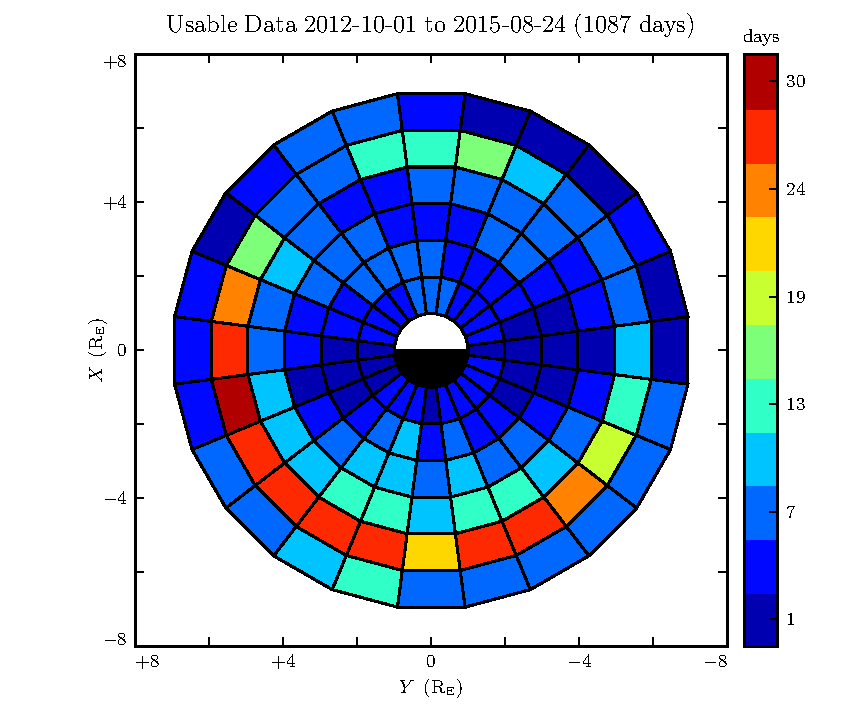
\includegraphics[width=\textwidth]{figures/pos_all_sharp.pdf}
  \caption[Distribution of Usable Van Allen Probe Data]{
    Three-dimensional electric field values are computed by assuming
    $\vec{E} \cdot \vec{B} = 0$. Data is discarded whenever the magnetic field
    falls within \SI{15}{\degree} of the spin plane, which introduces a bias
    against the flanks. Furthermore, the probes have completed one and a half
    precessions around Earth; the dayside has been sampled once at apogee, and
    the nightside twice. 
  }
  \label{fig_pos_all_sharp}
\end{figure}

Field measurements are transformed from GSE coordinates into the same dipole
coordinates used in \cref{ch_model,ch_results}. The \z axis (parallel to the
background magnetic field) is estimated using a ten-minute running average of
the magnetic field measurements. The \y axis is set parallel to
$\zhat \times \vec{r}$, where \vec{r} is the probe's geocentric position
vector. The \x axis is then defined per $\xhat \equiv \yhat \times \zhat$. This
scheme guarantees that the axes are right-handed and pairwise
orthogonal\cite{liu_2009}. 

The \about1000 days of usable data are considered half an hour at a time, which
gives a frequency resolution of \about\SI{0.5}{\mHz} in the discrete Fourier
transform. Spectra are computed for all six field components: \dft{B_x},
\dft{B_y}, \dft{B_z}, \dft{E_x}, \dft{E_y}, and \dft{E_z}. The background
magnetic field is subtracted before transforming the magnetic field components,
leaving only the perturbation along each axis\footnote{As in
\cref{ch_math,ch_model,ch_inertia,ch_results}, $B_x$, refers not to the full
magnetic field in the \x direction, but to the perturbation in the \x direction
from the zeroth-order magnetic field. The same is true for $B_y$ and $B_z$. }.
Each waveform is also shifted vertically so that its mean over the thirty
minute event is zero. 

Frequency-domain Poynting flux is computed from the electric and magnetic field
transforms. A factor of $L^3$ compensates the compression of the flux tube, so
that the resulting values are effective at the ionosphere. Poloidal and
toroidal Poynting flux, respectively, are given by:
\begin{align}
  \dft{S_P} &\equiv -\frac{L^3}{\mz} \dft{E_y} \dft{B_x^*} &
  \dft{S_T} &\equiv  \frac{L^3}{\mz} \dft{E_x} \dft{B_y^*}
\end{align}

The poloidal and toroidal channels are independently checked for Pc4 waves. For
each channel, a Gaussian profile is fit to the magnitude of the Poynting flux,
$|\dft{S}\arg{\omega}|$. If the fit fails to converge, or if the peak of the
Gaussian does not fall within \SI{5}{\mHz} of the peak value of \dft{S}, the
event is discarded. Events are also discarded if their frequencies fall outside
the Pc4 frequency range (\SIrange{7}{25}{\mHz}) or if their amplitudes fall
below \SI{e-2}{\mW/\m\squared} (out of consideration for instrument
sensitivity). 

Events are discarded if their parity is ambiguous. The electric field and the
magnetic field must be coherent at a level of 0.9 or better (judged at the
discrete Fourier transform point closest to the peak of the Gaussian fit). Any
event within \SI{3}{\degree} of the magnetic equator is also not used; as
discussed in \cref{ch_flrs}, in order to distinguish an odd mode from an even
mode, it's necessary to know whether the observation is made north or south of
the equator. 

%\todo{How much time do the probes spend within \SI{3}{\degree} of the magnetic equator? }

A visual inspection of events shows that those with broad ``peaks'' in their
spectra are typically not peaked at all --- they are noisy spectra with several
spectral features grouped just closely enough to trick the fitting routine. A
threshold is set at a FWHM of \SI{3}{\mHz} (equally, a standard deviation of
\SI{1.27}{\mHz}). Any event with a Gaussian fit broader than that is discarded.

Notably, events are not filtered on their phase --- that is, on the division of
their energy between standing and traveling waves. This is the topic of
\cref{sec_phase}. 

%\todo{Are we biased in terms of \DST? What's the distribution look like for the good data and for the bad data? }

% -----------------------------------------------------------------------------
% -----------------------------------------------------------------------------
% -----------------------------------------------------------------------------
\section{Events by Mode}
  \label{sec_rate}

The filters described in \cref{sec_selection} yield 762 Pc4 events, the spatial
distribution of which is shown in \cref{fig_rate_all_sharp}. In each bin, the
event count is normalized to the amount of usable data
(\cref{fig_pos_all_sharp}). Bins shown in white contain zero events. The rate
in the bottom corner is an overall mean; it's an estimate of how often Pc4
events would be observed if the sampling were distributed uniformly in space.

\begin{figure}[!htb]
  \centering
  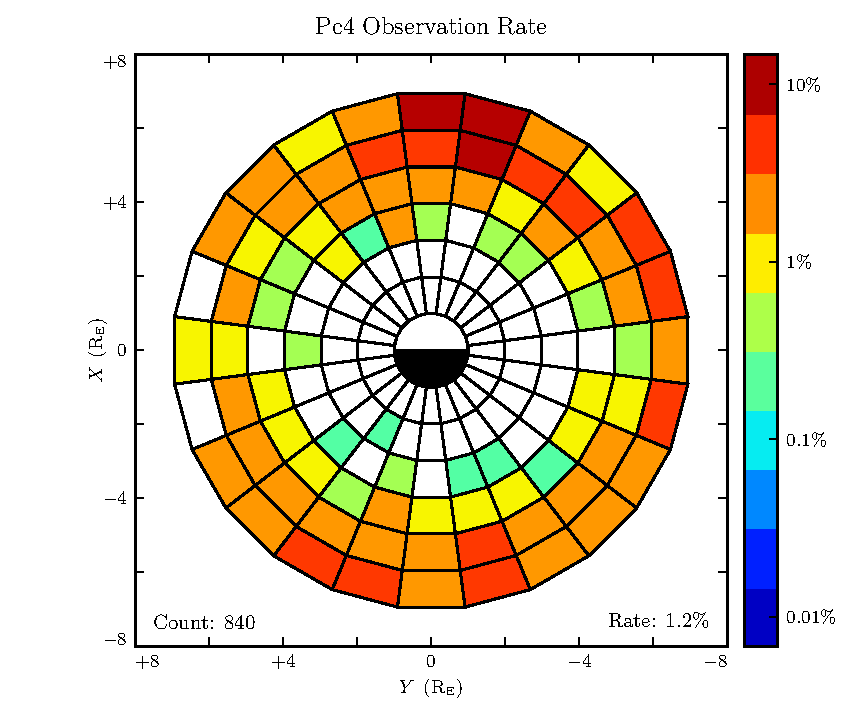
\includegraphics[width=\textwidth]{figures/rate_all_sharp.pdf}
  \caption[Rate of Pc4 Events]{
    The above figure shows the spatial distribution of all 762 observed Pc4
    events. Counts are normalized by the amount of usable data in each bin. The
    value in the bottom-right corner is the mean of the rate in each bin, with
    the rate in each bin weighed by the area of that bin. Events where the
    poloidal and toroidal channel both trigger (\about\SI{10}{\percent} of
    events) are counted as only a single event. Bins shown in white contain
    zero events. 
  }
  \label{fig_rate_all_sharp}
\end{figure}

Consistent with previous work, Pc4 events peak on the dayside and are rarely
observed at $L < 4$. Nearly \SI{30}{\percent} of the usable data shown in
\cref{fig_pos_all_sharp} is taken at $L < 4$, yet only 16 of the 762 events
(\SI{2}{\percent}) appear there. 

On the other hand, the present work runs contrary to Dai's 2015 result in terms
of Pc4 event rates with respect to the plasmapause (not shown). His analysis
found (poloidal) Pc4 pulsations to be comparably common inside and outside the
plasmapause\cite{dai_2015}. In the present work, only 40 of the 762 events
(\SI{5}{\percent}) fall inside the plasmasphere, despite the fact that
\SI{40}{\percent} of the available data falls within the plasmasphere. The
disparity is not likely due to a difference in sampling --- Dai's work, like
the present work, uses data from the Van Allen Probes mission. Rather, the
difference is likely due to a difference in how the plasmapause is defined. Dai
identifies the plasmapause by the maximum gradient in electron number density,
while the present work takes an electron density of \SI{100}{\percc} to mark
the plasmapause\footnote{Per ongoing work by Thaller. }. 

The same events in \cref{fig_rate_all_sharp} are shown again in
\cref{fig_mode_all_sharp}, partitioned by polarization and parity. 

\begin{figure}[!htb]
  \centering
  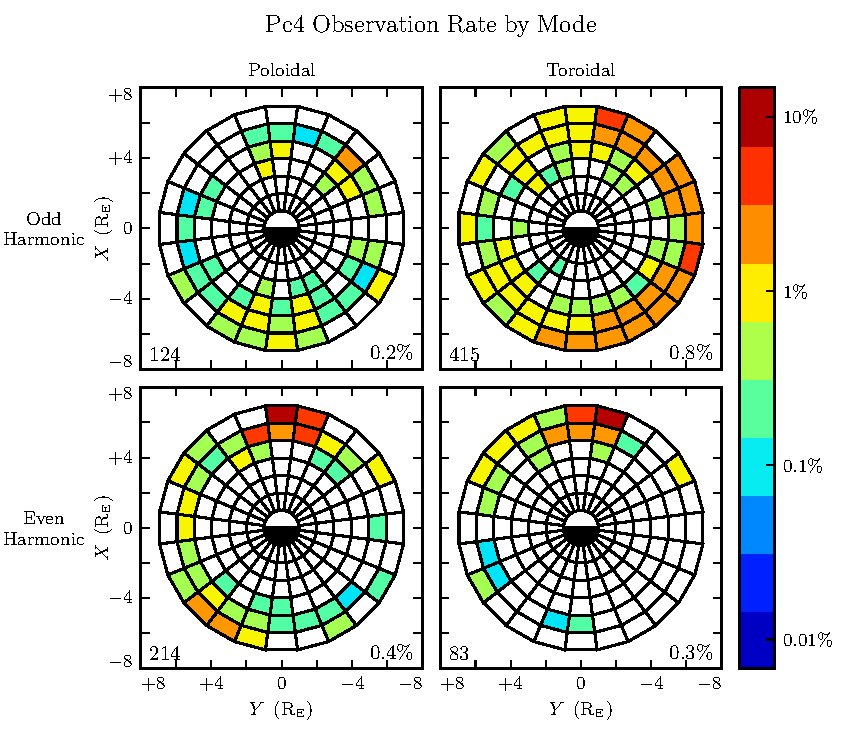
\includegraphics[width=\textwidth]{figures/mode_all_sharp.pdf}
  \caption[Rate of Pc4 Events by Mode]{
    The above figure shows the spatial distribution for the same 762 events
    shown in \cref{fig_rate_all_sharp}, partitioned by polarization and parity.
    The selection criteria described in \cref{sec_selection} ensure that both
    properties are known for all events. Event counts are normalized by the
    time spent by the amount of usable data in each bin. Counts shown in the
    bottom-left corners do not sum to 762 because some events trigger on both
    the poloidal channel and the toroidal channel. 
  }
  \label{fig_mode_all_sharp}
\end{figure}

The distribution of even poloidal events in \cref{fig_mode_all_sharp} is
consistent with that reported by Dai\cite{dai_2015}: the observation rate is
peaked at noon, and smeared across the dusk side. Notably, Dai's work focused
on even poloidal waves. While he did not explicitly remove odd events from his
sample, he did introduce a threshold in the magnetic field. This threshold is
preferrentially satisfied by even waves (which have a magnetic field antinode
near the equator) compared to odd waves (which have a magnetic field node). Dai
characterized the parity of only a quarter of his events; among those, he found
even harmonics to outnumber odd harmonics ten-to-one. 

In fact --- to the degree that they can be straightforwardly compared --- the
distributions in \cref{fig_mode_all_sharp} also show agreement with work by
Anderson\cite{anderson_1990} (using AMPTE/CCE), Kokubun\cite{kokubun_1989}
(using ATS6), Liu\cite{liu_2009} (using THEMIS), and Motoba\cite{motoba_2015}
(using GOES). Toroidal events dominate overall, and are primarily seen on the
morning side. Poloidal events are spread broadly in MLT, with a peak near noon
and odd harmonics in the early morning. 

Crucially, the present work can offer insight into how previous results fit
together. Unlike events considered in previous works, those shown in
\cref{fig_mode_all_sharp} have all been categorized in terms of both
polarization and parity. And, crucially, the selection process has not
introduced a bias with respect to polarization or parity (at least not an
obvious one). 

The even events shown in \cref{fig_mode_all_sharp} show good agreement with the
numerical results in \cref{ch_results}. The even poloidal and even toroidal
distributions are qualitatively similar, as might be expected if even poloidal
waves served as a source for even toroidal waves. Even poloidal waves are more
prevalent, suggesting a typical event duration comparable to the
poloidal-to-toroidal rotation timescale. And even toroidal events are skewed
dayward compared to even poloidal events, suggesting that poloidal-to-toroidal
rotation is inhibited by increased Joule dissipation on the nightside. 

The same can be said to some extent for the odd events in
\cref{fig_mode_all_sharp}, though the trends are less strong. Odd poloidal and
odd toroidal events are both scarce on the dusk flank. On the dawn flank,
poloidal events skew nightward, while toroidal events are spread broadly ---
that is, they are skewed dayward compared to the poloidal events. However, it's
unclear why odd toroidal events outnumber odd poloidal events to such a degree. 

When the 762 events are broken down by mode in \cref{fig_mode_all_sharp}, the
result is 124 odd poloidal events, 214 even poloidal events, 415 odd toroidal
events, and 83 even toroidal events --- a total of 836 events. The total is
greater than 762 because in \about\SI{10}{\percent} of events, the poloidal and
toroidal channels trigger independently. Such cases are marked as a single
event in \cref{fig_rate_all_sharp}, but the toroidal and poloidal events are
both shown in \cref{fig_mode_all_sharp}. 

Double-triggering can be taken as a vague proxy for event quality. When the
channels both trigger independently, the two events almost always (71 of 74
events) exhibit the same parity. This suggests a poloidal wave with suffient
power, and a sufficient narrow spectral peak, that it can still be seen after
much of its energy has rotated to the toroidal mode. 

\begin{figure}[!htb]
  \centering
  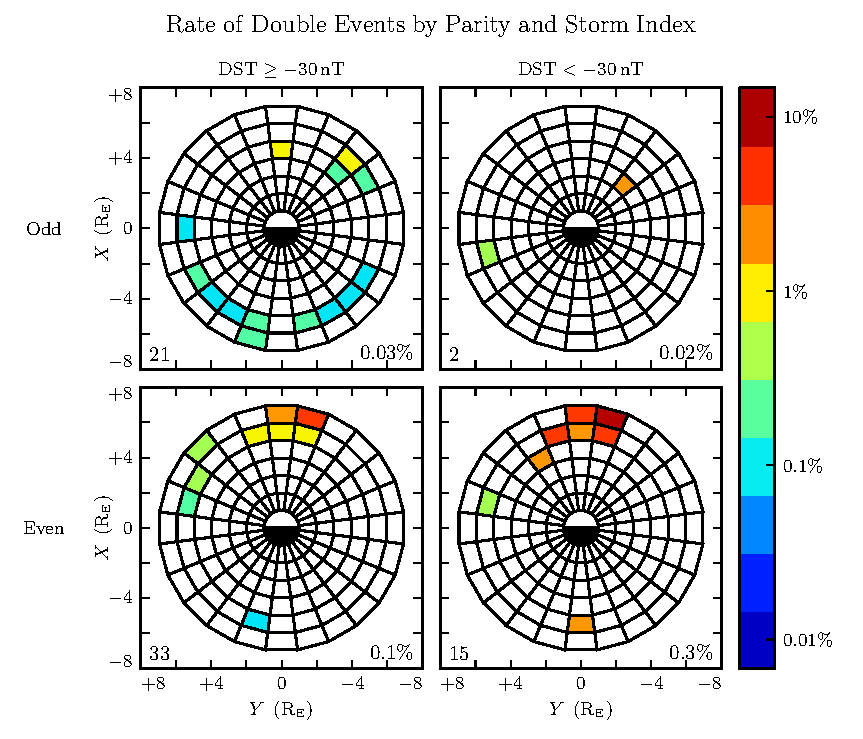
\includegraphics[width=\textwidth]{figures/double_rate_sharp.pdf}
  \caption[Rate of Double Pc4 Events by Parity and Storm Index]{
    A double event is a simultaneous triggering of the poloidal and toroidal
    channels on the same probe. In such cases, the two channels almost always
    exhibit the same parity. Double events serve as a vague proxy for event
    quality --- a poloidal event with sufficient strength and clarity to be
    seen even after much of its energy has rotated to the toroidal mode. Odd
    double events are spread broadly; even events are concentrated near noon,
    and become more common during geomagnetically active times. 
  }
  \label{fig_double_rate_sharp}
\end{figure}

The spatial distribution of double events is shown in
\cref{fig_double_rate_sharp}. The left column shows events observed with
$\DST \geq \SI{-30}{\nT}$, normalized by the amount of usable data at
$\DST \geq \SI{-30}{\nT}$. The right column shows events at
$\DST < \SI{-30}{\nT}$, normalized by the amount of data with
$\DST < \SI{-30}{\nT}$. 

Odd double-triggering events are spread broadly in MLT. They rarely occur twice
on the same day; the 23 events shown take place over 20 different dates. Odd
double events occur at similar rates regardless of \DST. 

Even-harmonic double-triggering events, on the other hand, are mostly seen near
noon, and are significantly more common during geomagnetically active times.
Even events are also more concentrated than odd ones. The 48 even-harmonic
double-events shown in the bottom row of \cref{fig_double_rate_sharp} are
spread over 20 days, and 35 of them are spread over just 7 days. This
clustering --- where the poloidal and toroidal channel both trigger for five to
ten half-hour events in the same day --- is prevalent regardless of \DST. 

%Not only does \cref{fig_mode_all_sharp} show that toroidal events outnumber poloidal events, but it also shows that toroidal events are predominantly odd harmonics --- as opposed to the primarily-even poloidal events. 

%This may suggest that odd poloidal waves are more likely than even ones to be driven at low modenumber (allowing a prompt rotation of that energy to the toroidal mode). One might expect low-\azm poloidal modes to be driven by a broad, sudden change in solar wind dynamic pressure, for instance. The relative scarcity of odd poloidal observations on the dayside may indicate a short-lived source. At low \azm, energy rotates to the toroidal mode on the order of a wave period; without an ongoing source, there would be no poloidal wave to observe. 

%\todo{Actually, it looks like odd poloidal waves are split about half-and-half around $\left| \frac{B_z}{B_x} \right| = 0.2$. Compressional odd modes are more common near midnight. Noncompressional ones are mostly in the morning. Even poloidal events are skewed toward low \azm. This is probably worth showing. }

%\todo{Odd poloidal events are skewed nightward compared to odd toroidal events. This is not surprising. Per \cref{ch_results}, nightside poloidal events are less likely to give rise to toroidal events than those on the dayside. Even events too, actually. The toroidal distribution looks like the poloidal distribution, but skewed dayward. }

%This would furthermore be consistent with even modes' apparent dearth of ground signatures\cite{takahashi_1992}. If even harmonics tend to be produced at higher modenumber than odd ones, even harmonics would be expected to produce ground signatures less often\footnote{See \cref{attenuation}. }. 

%Even poloidal modes and even toroidal modes exhibit similar distributions in space: both are peaked at noon and smeared across the dusk flank, with little activity on the dawn side. This is further support for the even poloidal wave as a significant source for the even toroidal mode. 

%\todo{Conventional explanation for dawn-dusk asymmetry. }

%\todo{What else do we want to say here? Or does the rest of the commentary belong in the later sections? Note that plots in future sections are lower resolution, to make sure that the number of bins remains much smaller than the number of events. }

%\todo{How does this relate to the numerical results in \cref{ch_results}? }

%Dai\cite{dai_2015} used RBSP to look at poloidal Pc4 events, with a bias in favor of the second harmonic --- 890 events. Events are most common near noon, but are spread across the day and dusk side, with a few stragglers at midnight. 

%Anderson\cite{anderson_1990} used AMPTE/CCE (mostly $L>7$, near the equator) to look at Pc4 events --- 7000 hours. Limited commentary on parity. Toroidal modes were found to outnumber poloidal modes three-to-one. ``Harmonic toroidal resonances'' are spread 0600 to 1600. ``Fundamental toroidal resonances'' (which are not mutually exclusive with harmonic ones!) appear everywhere but dusk. 

%Liu\cite{liu_2009} used THEMIS (equatorial orbit, $L$ out to \about10) to look at both poloidal and toroidal modes --- 9805 one-minute Pc4 events (?). No commentary on parity. Poloidal events are most common at noon (with another peak post-midnight) and strongest on the dusk side. Toroidal events are most common from pre-dawn to pre-noon and strongest pre-midnight and post-dawn. 

%Kokubun\cite{kokubun_1989} used ATS6 (synchronous orbit) --- \about150 events. No commentary on harmonic. Toroidal events dominate in the dawn sector. Poloidal events are spread across all MLT, with a peak in the early afternoon and Pgs in the early morning. 

%Motoba\cite{motoba_2015} used GOES13 and GOES15 (geosynchronous) to look specifically at Pgs --- 105 events. Seen from midnight to noon, with a strong peak before dawn, 0300 or so. 

%\todo{Even poloidal events and even toroidal events are distributed similarly, which is good to see, since even poloidal events give rise to even toroidal events. The relationship is less clear for odd events, though odd poloidal modes and odd toroidal modes are both least common at dusk. }

%\todo{Odd toroidal events are by far the most commonly observed. Oddly, even poloidal events are the least common. }

%\todo{Even modes are less likely to be observed on the ground? \cite{takahashi_1992} }

% -----------------------------------------------------------------------------
% -----------------------------------------------------------------------------
% -----------------------------------------------------------------------------
\section{Events by Amplitude}
  \label{sec_amp}

One might reasonable be concerned that the spatial distributions presented in
\cref{fig_mode_all_sharp} are dominated by these small events, while Pc4 events
large enough to be noteworthy follow a different distribution entirely. 

\begin{figure}[!htb]
  \centering
  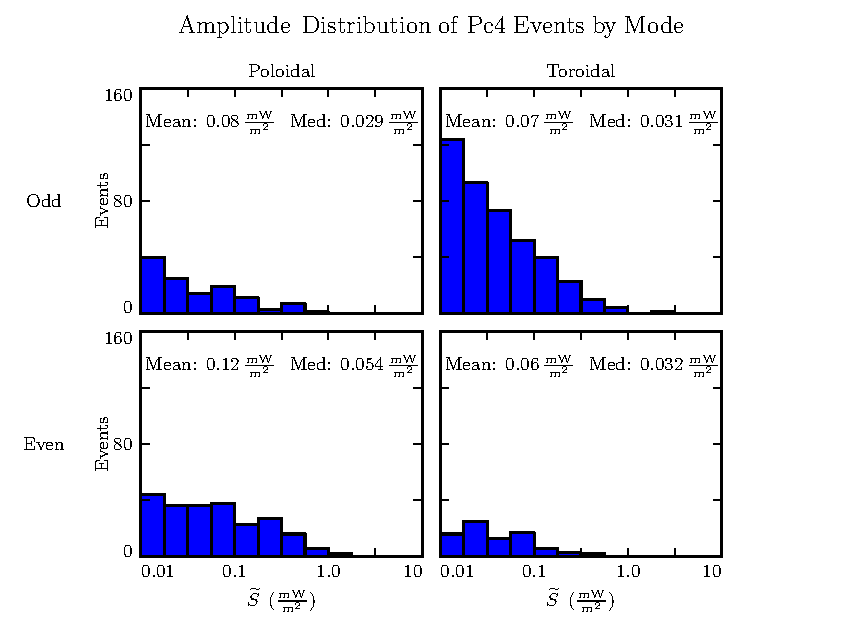
\includegraphics[width=\textwidth]{figures/amp.pdf}
  \caption[Amplitude Distribution of Pc4 Events by Mode]{
    Amplitude distribution is shown for Pc4 events by parity and polarization,
    based on the peak of the spectrum's Gaussian fit. Odd poloidal events, odd
    toroidal events, and even toroidal events fall off sharply with increasing
    amplitude, while the even poloidal events are distributed more broadly ---
    the mean and median of the even poloidal distribution are twice as large as
    those of the others. 
  }
  \label{fig_amp}
\end{figure}

The distribution of event magnitudes is presented in \cref{fig_amp}, graded
based on the peak of the Gaussian fit of each event's Poynting flux,
$|\dft{S}\arg{\omega}|$. Mean and median values are listed for each mode. Most
events are small, with Poynting flux well below \SI{0.1}{\mW/\m\squared} when
mapped to the ionosphere. Only a handful of events --- 3 out of 762 --- exceed
\SI{1}{\mW/\m\squared}, typically taken to be the threshold at which visible
auroral arcs form. 

%One such event is shown in \cref{fig_sample_event_strong}. 

%\todo{Say something about this event? Not really clear what purpose is served by this example, actually. As a matter of curiosity, the apparent wave activity in the toroidal channel did not pass the event selection trigger because the electric and magnetic waveforms are not coherent. }

Perhaps the most notable feature of \cref{fig_amp} is the relative uniformity
of the distribution of even poloidal events. If a higher magnitude threshold is
imposed, as shown in \cref{fig_mode_amp}, the proportion of even poloidal
events rises. 

The spatial bins in \cref{fig_mode_amp} are larger than those in
\cref{sec_rate}; this change reflects an effort to keep the number of events
large compared to the number of bins, even when considering relatively small
subsets of the data. The larger bins --- two hours wide in MLT and divided at
$L = 5$ radially --- are also used in \cref{sec_f,sec_phase}. All of the
large-binned bullseye plots also share a common logarithmic color bar. 

All else being equal, one might expect the amplitude distribution of even
toroidal events to mimic that of even poloidal events, since poloidal waves
asymptotically rotate to toroidal waves. However, this does not seem to be the
case. The mean and median magnitudes are more or less consistent for even
toroidal events, odd toroidal events, and odd poloidal events, while even
poloidal events are twice as large by those metrics. This would seem to imply
that large even poloidal modes have disproportionately high modenumbers, and
thus deliver energy to the toroidal mode less efficiently. This explanation
is unsatisfying, however; \cref{fig_mode_amp} shows that even poloidal and
toroidal modes both become more concentrated near noon at high amplitude,
suggesting a common origin. 

%\begin{figure}[!htb]
%  \centering
%  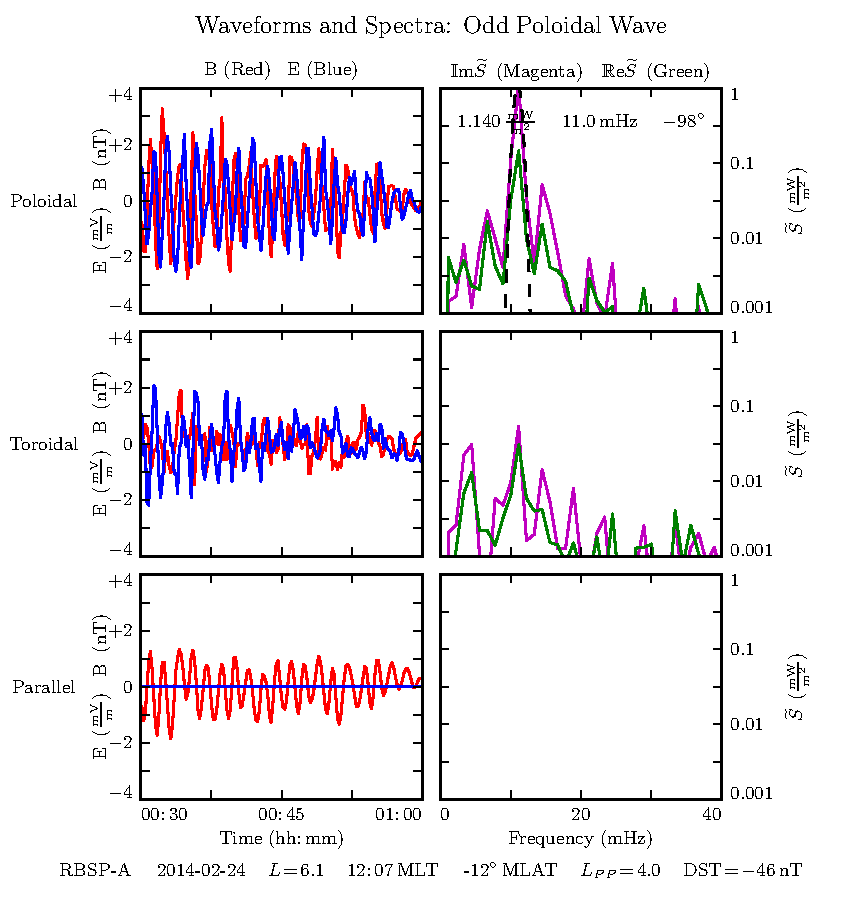
\includegraphics[width=\textwidth]{figures/sample_event_strong.pdf}
%  \caption[Waveforms and Spectra for a Strong Pc4 Event]{
%    \todo{$\cdots$}
%  }
%  \label{fig_sample_event_strong}
%\end{figure}

\begin{figure}[!htb]
  \centering
  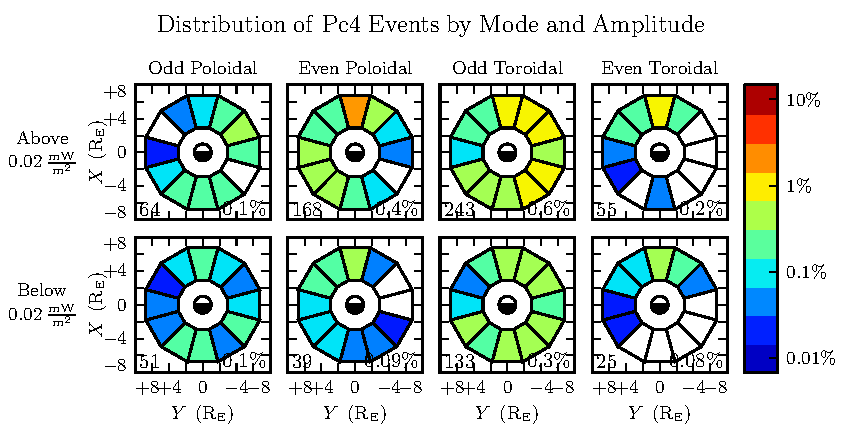
\includegraphics[width=\textwidth]{figures/mode_amp.pdf}
  \caption[Rate of Pc4 Events by Mode and Amplitude]{
    The above figure shows the distribution of Pc4 event observations by mode.
    Event magnitude cutoff is constant down each column, and increases from
    left to right. Stronger even events appear to become more concentrated on
    the dayside as the amplitude increases. Even poloidal events also become
    significantly more numerous relative to the other three modes, from
    \SI{26}{\percent} at a cutoff of \SI{0.01}{\mW/\m\squared} to
    \SI{41}{\percent} above \SI{0.1}{\mW/\m\squared}. 
  }
  \label{fig_mode_amp}
\end{figure}

% -----------------------------------------------------------------------------
% -----------------------------------------------------------------------------
% -----------------------------------------------------------------------------
\section{Events by Frequency}
  \label{sec_f}

The difference in magnetospheric conditions between the dayside and the
nightside suggest that different eigenfrequencies should arise between dayside
and nightside resonances at the same $L$-shell. In fact, this phenomenon has
been observed directly; the frequencies of azimuthally-drifting FLRs have been
shown to change over time\cite{motoba_2015}. The effect is attributed to the
difference in mass loading (and thus \Alfven speed) as a function of MLT. 

This effect was furthermore apparent in the numerical results shown in
\cref{ch_results}, where \Alfven speeds on the dayside (based on empirical
profiles) gave rise to significantly higher eigenfrequencies than those on the
nightside. 

In \cref{fig_mode_f}, events at \SIrange{11}{17}{\mHz} (center column) do seem
to be shifted nightward compared to those at \SIrange{7}{11}{\mHz} (left
column), but the effect is far less pronounced than what is suggested by
\cref{sec_day,sec_night}. 

\begin{figure}[!htb]
  \centering
  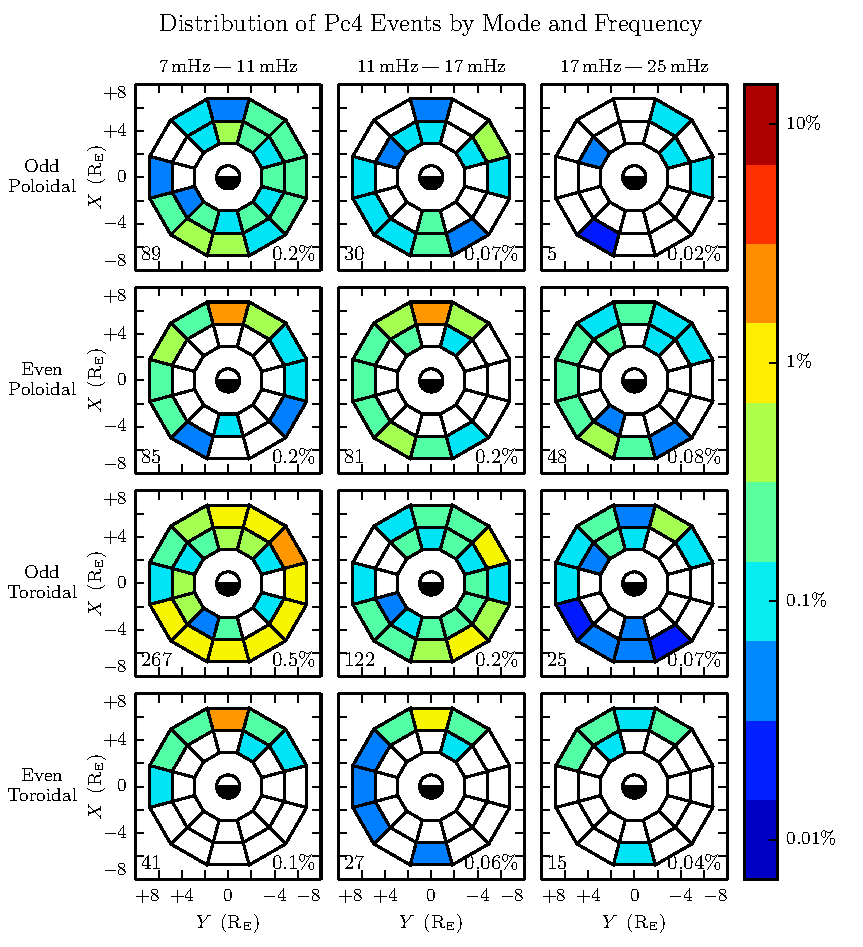
\includegraphics[width=\textwidth]{figures/mode_f.pdf}
  \caption[Rate of Pc4 Events by Mode and Frequency]{
    Event distributions above are shown in terms of mode (row) as well as event
    frequency (column). Mid-frequency Pc4 events are shifted somewhat nightward
    compared to low-frequency Pc4 events, as might be expected from the
    dayside's faster \Alfven speed. At the top of the Pc4 band, the
    distribution of odd toroidal events takes on a decidedly different
    character; this is likely because these events are third harmonics rather
    than first harmonics. 
  }
  \label{fig_mode_f}
\end{figure}

%\todo{We should show the runs driven at $L\sim5$ across the board. Dayside and nightside. That way we can make a fair comparison. }

As might be expected, even events are more prevalent than (mostly fundamental)
odd events higher in the Pc4 range. Events at \SIrange{7}{11}{\mHz} (left
column) outnumber those at \SIrange{17}{25}{\mHz} (right column) ten-to-one or
more for odd events. Among even events, the comparison is more like
three-to-one. 

The spatial distribution of odd toroidal events above \SI{17}{\mHz} warrants
specific consideration. Whereas odd toroidal events overall show an
overwhelming preference for the morning side, those at the top of the Pc4
frequency band instead appear from noon to dusk. It's possible that this
distribution is a consequence of the small number of events (25). More likely,
however, is that these are third-harmonic events, and that their source more
closely resembles the source for second-harmonic waves than it does first
harmonics. 

%\todo{Have people looked at third harmonics? }

The frequency distribution for each mode is shown in \cref{fig_f}. The most
distinctive feature, certainly, is the frequency peak in the odd toroidal mode
near \SI{9}{\mHz}. This is in line with the idea that toroidal waves exhibit
frequencies that depend sharply on $L$, as discussed in \cref{ch_results}.
While the Van Allen Probes' orbits do cover a large range of $L$-shells, their
observations (and thus the selected events) are concentrated near apogee at
$L \sim 6$. 

\begin{figure}[!htb]
  \centering
  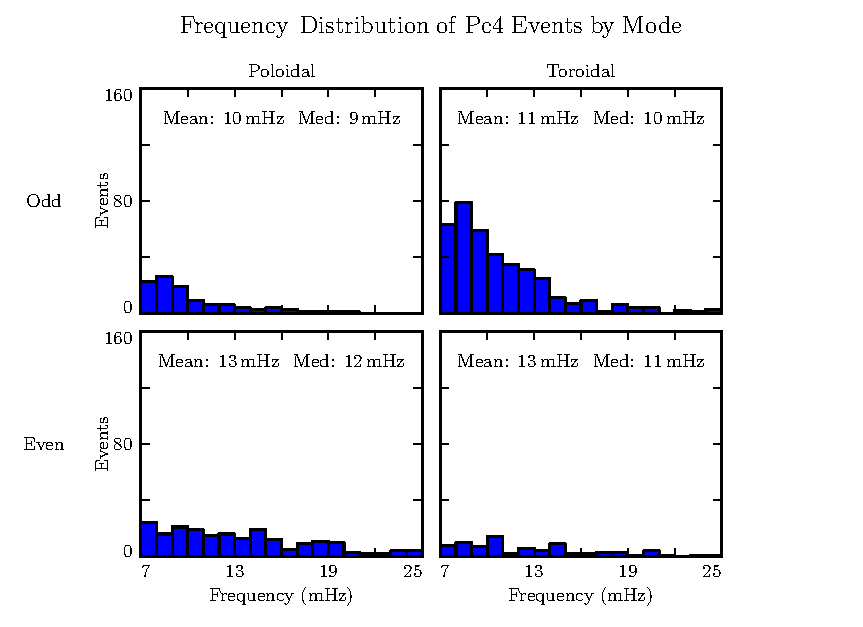
\includegraphics[width=\textwidth]{figures/f.pdf}
  \caption[Frequency Distribution of Pc4 Events by Mode]{
    Frequency distributions are shown for all events, divided by harmonic and
    polarization. Odd toroidal events exhibit a particularly sharp peak in
    frequency, which is consistent with the toroidal mode's strong correlation
    with the local eigenfrequency. Poloidal modes appear more spread out in
    frequency, which is also consistent with past observations and with the
    numerical results in \cref{ch_results}. 
  }
  \label{fig_f}
\end{figure}

%\todo{Maybe put the Gaussian fit back on top of these distributions? The distributions are not particularly Gaussian, but it gives a quantitative estimate of the spread. }

% -----------------------------------------------------------------------------
% -----------------------------------------------------------------------------
% -----------------------------------------------------------------------------
\section{Events by Phase}
  \label{sec_phase}

The phase of a wave --- that is, the phase offset between a wave's electric and
magnetic fields --- indicates how its energy is partitioned between the
standing and traveling wave modes. An ideal standing wave has a phase of
$\pm$\SI{90}{\degree}, and thus its Poynting flux is completely imaginary. A
traveling wave, on the other hand, has electric and magnetic fields in phase
(or in antiphase), and is associated with a net movement of energy, usually
toward the ionosphere. 

Wave phase is a topic of significant interest, since it allows an estimate to
be made of the wave's lifetime. And, because phase can only be determined using
simultaneous electric and magnetic field measurements, it has only recently
become observable. 

%\todo{Do people really care about phase, or is it just John? }

The energy per unit volume, and the rate at which energy is carried out of that
volume by Poynting flux, are respectively given by:
\begin{align}
  \label{def_phase}
  U &= \frac{R^3}{2\mz} B^2 &
  \ddt U &= \frac{R^2}{\mz} E B \cos\varphi
\end{align}

Where $B$, $E$, and $R$ are the characteristic magnetic field magnitude,
electric field magnitude, and length scale. The phase,
$\varphi \equiv \arctan\frac{ \imag\dft{S} }{ \real\dft{S} }$, enters because
only real Poynting flux carries energy. 

The ratio of the two quantities in \cref{def_phase} gives a characteristic
timescale over which energy leaves the system
\begin{align}
  \label{def_tau}
  \tau &\equiv \frac{BR}{2 E \cos\varphi}
\end{align}

In the present case, magnetic fields are on the order of \SI{1}{\nT} and
electric fields are on the order of \SI{1}{\mV/\m}. A reasonable scale length
might be \SI{e4}{\km}, the distance traversed by the probe over the course of
a half-hour event near apogee (notably, back-to-back events are unusual). 

At a phase of \SI{80}{\degree}, this timescale is comparable to a Pc4 wave
period. At \SI{135}{\degree}, where energy is divided evenly between the
standing and traveling wave, the timescale is just 7 seconds. A wave with a
phase so far from \SI{90}{\degree} would quickly vanish unless it were
constantly being replenished. 

An example of just such an event is shown in \cref{fig_sample_event_phase}.
The left column shows electric and magnetic field waveforms in blue and red
respectively. The right shows the corresponding spectra: imaginary Poynting
flux in magenta (corrresponding to the strength of the standing wave) and real
Poynting flux in green (for the traveling wave). The black line is a Gaussian
fit to the magnitude of the Poynting flux. 

The poloidal channel shows a mostly-standing wave, with a phase of
\SI{79}{\degree}. The coherent activity in the compressional magnetic field
implies a low azimuthal modenumber, and thus a fast rotation of energy from the
poloidal mode to the toroidal mode. It's likely the rotation of energy from the
poloidal mode contributes significantly to the toroidal mode's lifetime; the
toroidal wave's phase is \SI{130}{\degree}, so its energy should be carried
away quickly by Poynting flux. 

\begin{figure}[!htb]
  \centering
  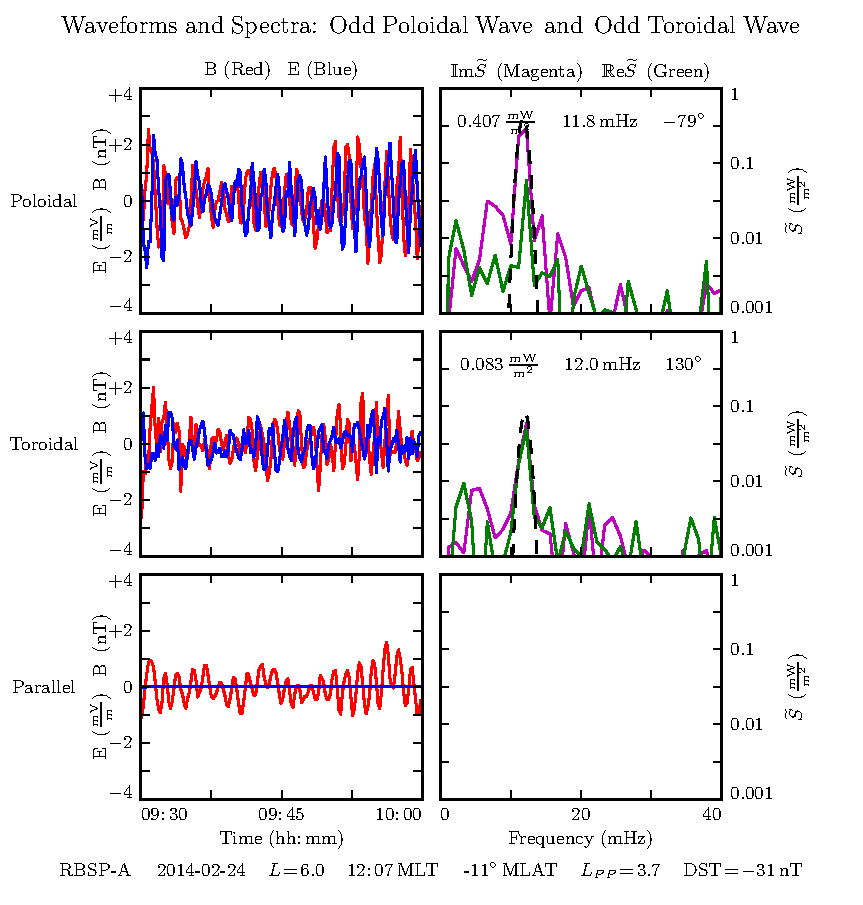
\includegraphics[width=\textwidth]{figures/sample_event_phase.pdf}
  \caption[Waveforms and Spectra for a Pc4 Event]{
    The above is a double event, where the poloidal and toroidal channels have
    been independently selected as events. The poloidal channel shows a wave
    with most of its energy in the standing wave (phase of \SI{79}{\degree}).
    The toroidal mode has a significant traveling component (phase of
    \SI{130}{\degree}). The compressional activity implies a low modenumber,
    which would cause energy to rotate quickly from the poloidal mode to the
    toroidal mode --- evidently at a sufficient rate to replenish the losses
    due to the traveling mode's real Poynting flux. 
  }
  \label{fig_sample_event_phase}
\end{figure}

The selection process described in \cref{sec_selection} does not explicitly
consider phase. However, the discrete Fourier transform is performed over a
half-hour time span. An event with a comparatively short lifetime would be
unlikely to register. It's unsurprising to see the events in \cref{fig_phase}
are tightly clustered near \SI{90}{\degree}. 

\begin{figure}[!htb]
  \centering
  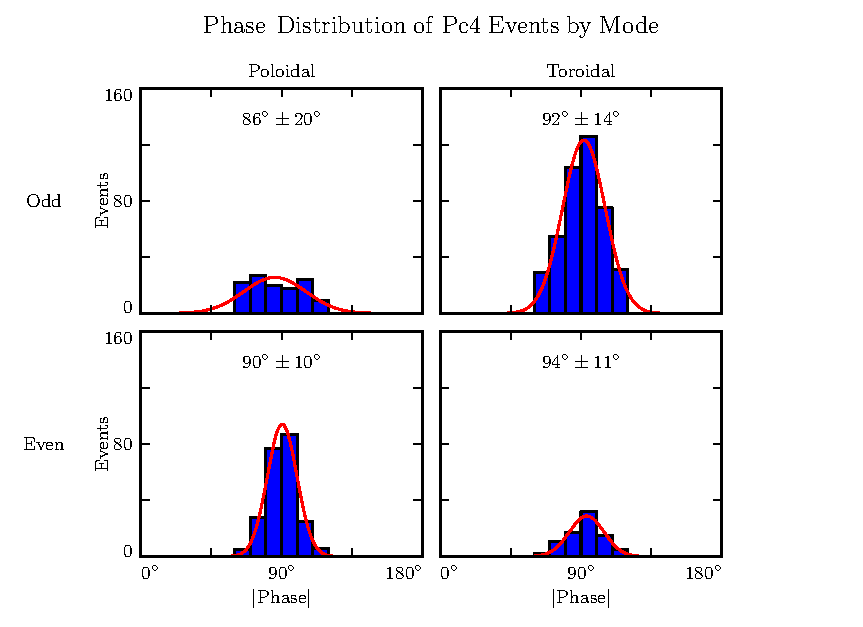
\includegraphics[width=\textwidth]{figures/phase.pdf}
  \caption[Phase Distribution of Pc4 Events by Mode]{
    The (absolute) phase of the selected Pc4 events is shown above. All modes
    show phase distributions peaked around \SI{90}{\degree}. This reflects the
    fact that a significant traveling wave component quickly carries energy
    away from an FLR. Odd events are spread more broadly in phase than even
    events. This is consistent with the odd modes' electric field antinode near
    the equator, where events are observed; the characteristic loss timescale
    depends on $\frac{B}{E}$ per \cref{def_tau}. 
  }
  \label{fig_phase}
\end{figure}

It's further notable in \cref{fig_phase} that the odd events are more spread
out in phase than the even events. Near the equator, odd modes have an electric
field antinode and a magnetic field node; per \cref{def_tau}, an odd mode's
lifetime should be longer than that of an even mode with the same phase. 

Unlike amplitude (\cref{sec_amp}) and frequency (\cref{sec_f}), events of
different phase do not seem to exhibit different spatial distributions, as
shown in \cref{fig_mode_phase}. Comparisons are limited by the small event
counts in several of the subplots; however, coarsely speaking, events with
phases of \SI{75}{\degree} and worse (left column) show spatial distributions
more or less in proportion with events phased \SI{85}{\degree} or better (right
column). \cref{fig_phase} uses the absolute value of each event's phase, as
does \cref{fig_mode_phase}. 

\begin{figure}[!htb]
  \centering
  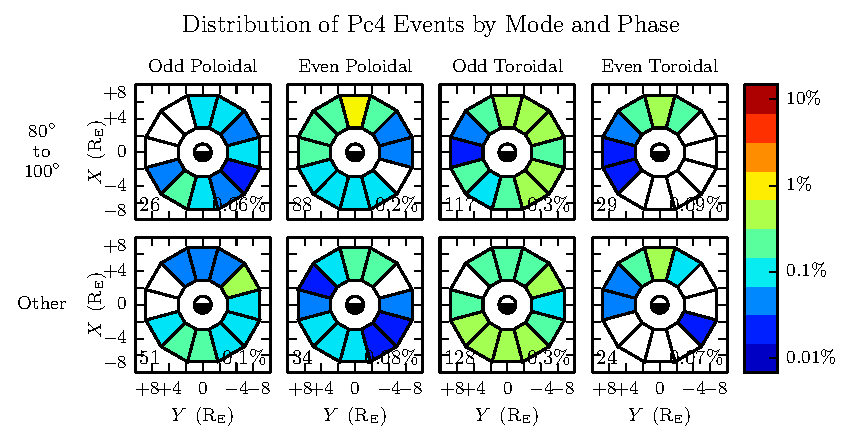
\includegraphics[width=\textwidth]{figures/mode_phase.pdf}
  \caption[Rate of Pc4 Events by Mode and Phase]{
    The observation rate of events is shown above, divided by (absolute) phase
    as well as mode. The closer a phase to \SI{90}{\degree}, the more of an
    event's energy is in the standing wave, rather than the traveling wave. The
    spatial distribution of events is more or less consistent between waves
    with phases very close to \SI{90}{\degree} and those with a significant
    traveling wave component. 
  }
  \label{fig_mode_phase}
\end{figure}

% -----------------------------------------------------------------------------
% -----------------------------------------------------------------------------
% -----------------------------------------------------------------------------
\section{Discussion}

The present chapter gives a survey of \about800 thirty-minute Pc4 events, each
characterized in terms of both parity and polarization, and selected in a way
that does not introduce an apparent bias in either property. No past study has
so thoroughly disentangled the parity and polarization of these waves.

Coarsely speaking, event distributions are found to be consistent with past
surveys. Toroidal events dominate overall, and are primarily seen on the
morning side. Poloidal events are spread broadly in MLT, with a peak near noon
and distinctive odd harmonics in the early morning. From there, the
simultaneous consideration of harmonic and polarization, combined with the
numerical results from \cref{ch_results}, offers significant insight. 

The near-noon peak of poloidal Pc4 events is shown to be due to even events (a
majority subset). Odd poloidal events occur preferrentially near midnight and
across the morning side. Similarly, toroidal events are mostly odd, and it is
specifically the odd toroidal events which occur on the morningside, while even
toroidal events peak near noon. 

The spatial distribution of even poloidal events looks much like the spatial
distribution of even toroidal events, except that the toroidal distribution is
skewed dayward compared to the poloidal. The same can be said of the odd
events. This is consistent (per \cref{ch_results}) with poloidal events as an
effective source for (same-parity) toroidal events on the dayside, and a
less-effective source on the nightside. 

Curiously, only a small minority (\SI{17}{\percent}) of toroidal events are
found to be odd, while a majority (\SI{63}{\percent}) of poloidal events are
even. This disparity may offer clues to the source of these waves. 

All events are found to follow a similar amplitude distribution, except for
even poloidal events, which are notably larger. The cause is unclear. 

The \about\SI{6}{\percent} of odd toroidal Pc4s at the top of the frequency
range (\SIrange{17}{25}{\mHz}) are found to exhibit a qualitatively different
spatial distribution from the rest. It's likely that these waves are third
harmonics, and that their excitation mechanism more closely resembles that of
second harmonics than it does first harmonics. 

Event phase is also considered. Most events of both polarizations are shown to
have absolute phase in the range \SIrange{80}{100}{\degree}, indicating that
the traveling component of Pc4 pulsations is small compared to the standing
component. Odd events are found to be spread more broadly in phase; this is
likely a consequence of being measured near the equator, where (due to the
electric field antinode) the lifetime of an odd event is significantly larger
than that of an even event with the same phase. 

% -----------------------------------------------------------------------------
% -----------------------------------------------------------------------------
% -----------------------------------------------------------------------------
%\section{Poloidal Pc4 Events by Compressional Coupling}

%\todo{Low-\azm poloidal Pc4 events are coupled to the compressional mode, while high-\azm ones are not. }

%\todo{The value of $\dft{B_z}/\dft{B_x} = 0.2$ comes from Dai\cite{dai_2015}. Can we match this up to an \azm value? Sounds like a job for Tuna! }

%\begin{figure}[!htb]
%    \centering
%    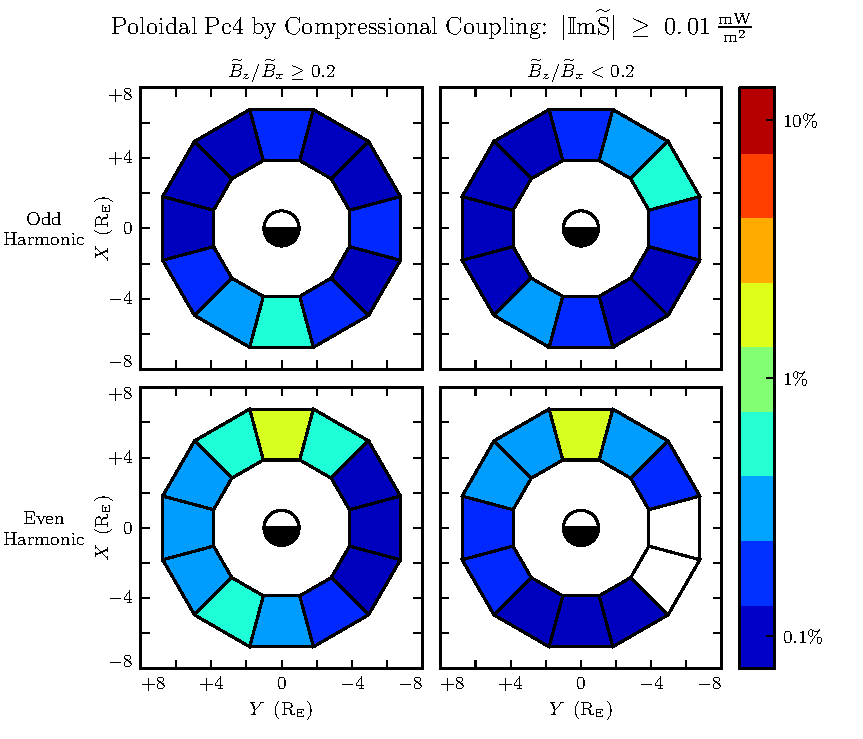
\includegraphics[width=\textwidth]{figures/azm_rate_all.pdf}
%    \caption[Poloidal Pc4 Rate by Compressional Coupling]{
%      \todo{Odd poloidal Pc4 events have a peak pre-noon and another peak near midnight. The pre-noon peak seems to be composed of high-\azm events, and the midnight peak seems to be low-\azm events. Low-\azm even poloidal events are spread broadly across the dusk side, while high-\azm even events are peaked strongly on the dayside --- consistent with Dai's results\cite{dai_2015}. }
%    }
%    \label{fig_azm_rate_all}
%\end{figure}




%\todo{Collections of events at a single ground observatory (near \SI{66}{\degree}) over significant periods of time: }

%Brekke\cite{brekke_1987} looked at 523 giant pulsation events recorded at Troms{\o}, Norway, from 1929 to 1985. This spanned several solar cycles. 

%Rolf\cite{rolf_1931} collected 28 events between 1921 and 1930 at Abisko. 

%Sucksdorf\cite{sucksdorff_1939} got 150 events between 1914 and 1938 in Sodankyl{\"a}. 

%Harang\cite{harang_1941}. 97 events from 1929 to 1941. Also Troms{\o}. Note that this may have been limited by the war! 

%This comes out to something like ... events over ... years. That's about ... giant pulsations per year, observed on the ground. 

%\todo{Collections of events at an array of ground observatories: }

%Chisham and Orr\cite{chisham_1991} found 34 events from 1984 to 1987 using the EISCAT magnetometer array in scandanavia. About \SI{5}{\degree} in MLT, decent coverage from \SIrange{63}{67}{\degree} mlat. This coincides with a solar minimum. 

%Motoba, in 2015, recorded 105 giant pulsation events. The observations were carried out by a number of ground magnetometers spanning $\sim \SI{90}{\degree}$ in local time and ranging roughly \SIrange{60}{70}{\degree} magnetic latitude\cite{motoba_2015}. This was mostly during a period of low solar activity, so we expect a high count. 

%\todo{Estimate of the size of an event's footprint:}

%Velkamp\cite{veldkamp_1960} looked at a single large event and showed that, at best, it was visible over a span of \SI{5}{\degree} in magnetic latitude. 

%This is seemingly consistent with the 29 February 2012 event discussed in detail by Motoba\cite{motoba_2015} --- Motoba shows some data, but doesn't discuss this aspect in detail. 

%Takahashi\cite{takahashi_2011} computes a FWHM of about 1 in L, or \SI{2}{\degree} magnetic latitude. 

%\todo{Tying that in to RBSP observations? }

%Note that it's a bit tricky to compare ground observations to in situ observations. Large-\azm events won't make it through the ionosphere. 

%There should be no bias with respect to MLT between a ground magnetometer and RBSP. Dai's analysis was specifically chosen to take advantage of the fact that RBSP's orbit had precessed all the way around the Earth. No preferred direction. And mlat shouldn't cause issues... these are FLRs, after all. 

%How strong does an event need to be on the ground, or in the sky, to count as a giant pulsation? Motoba 2015\cite{motoba_2015} has an event which tops out on the order of \SI{10}{\nT} on the ground. It's more like \SI{5}{\mV/\m} in situ. Takahashi\cite{takahashi_2011} has similar values. 

%If peak Pg observations are at $\SI{66}{\degree}$ mlat, that corresponds to $L = 6$. Then let's suppose that peak Pg viewing is $\SI{5}{\degree}$ wide --- estimating from the work of Velkamp and Motoba. That means RBSP should see lots of Pgs when it's between $L = 5.2$ andn $L = 7.1$. Well, \SI{7.1}{\RE} is outside its apogee, but the probes spend a fair amount of time outside $L = 5.2$, since they are moving pretty slowly at that point. 

%Giant pulsations have been shown to be more numerous in times of low solar activity. That was the whole point of Brekke's seminal 1987 paper, and it's consistent with what we show in \cref{ch_results}. The RBSP observations occur during peak solar times, though it's an anemic solar peak\cite{pesnell_2016}. 

%\todo{How much time does RBSP spend outside of $L = 5.2$ (for a range of \SI{5}{\degree})? How about $L = 5.6$ to $L = 6.5$ (for FWHM of \SI{2}{\degree}? }

%Each RBSP probe spends about \SI{30}{\percent} of its orbit between $L = 5.6$ and $L = 6.5$. 

%RBSP-A and RBSP-B count as two observers. In one $\sim 5$ cases out of hundreds do they simultaneously observe a poloidal Pc4 event (although, most notably for the 2012 event which \cite{dai_2013} considers in detail), both probes do fly through the same apparent event several hours apart from one another. 

%The duration of Dai's survey is October 2012 to June 2014. Scaled by 2 probes, each of which is present in the peak Pg lshells 30\% of the time, that comes out to almost exactly one year. 

%\todo{How many fundamental mode poloidal events do we see? How many could pass for giant pulsations? How many should we expect to see? }

%\todo{How weird is it for a fundamental mode poloidal Pc4 to be monochromatic? }

%\todo{How weird is it for a fundamental mode poloidal Pc4 to be stronger than \SI{5}{\mV/\m} at the equator? }






